\section{Markov decision processes}
The mathematical framework for reinforcement learning is the Markov decision process (MDP).
It can be considered as a generalisation of multi-armed bandits, where the agent observes a state before choosing an action, from which the reward probabilities — and now also state transition probabilities — depend.
More precisely, a Markov decision process is a tuple $M = (\mathcal{S}, \mathcal{A}, P, r)$.
The sets $\mathcal{S}$ and $\mathcal{A}$ are the state and action spaces, respectively, both of which may be infinite.
The transition probabilities $P(s' | s, a_t)$ are the probability of transitioning from state $s'$ to state $s$, given that action $a$ was taken.
Next, the reward function $r : \mathcal{S}^2 \times \mathcal{A} \to \mathbb{R}$ is a function that maps each transition and causing action to a real-valued reward.

The game is played similarly to a multi-armed bandit, in that the agent chooses an action at each time step $t$.
However, before each turn, the agent observes the current state $s_t \in \mathcal{S}$.
For the first turn, the state is taken from some distribution $P(s_0)$.
When the agent commits to an action $a_t \in \mathcal{A}$, the environment transitions to a new state $s_{t+1}$ according to the transition probabilities $P(s_{t+1} | s_t, a_t)$, and the agent receives a reward $r(s_t, a_t)$.

The goal is to find a (potentially probabilistic) policy which maps each state to an action, such that the agent receives the highest possible expected cumulative reward.
In particular, one attempts to maximise the expected future sum of discounted rewards, the return, defined as
\begin{equation}
    G_t = \mathbb{E} \left[ \sum_{\tau=0}^{\infty} \gamma^\tau X_{t+\tau} \right],
\end{equation}
where $X_t$ is the reward received at time $t$, $\gamma \in (0,1]$ is the discount factor.
The horizon $T$ may be infinite.
The discount factor is used to balance the importance of immediate rewards versus future rewards and to ensure convergence regardless of horizon finiteness.
In practice, $\gamma$ is a hyperparameter that is tuned to the problem at hand.

Hence, the optimal policy is given by the policy that maximises the expected return in starting state, namely
\begin{equation}
    \pi^* = \argmax_{\pi} \mathbb{E} \left[ G_0 \right],
\end{equation}
where the expectation is taken over the distribution of initial states.

Note that policies will in general depend on the whole history of states, actions and rewards, and not just the current state.

\begin{figure}
    \centering
    \begin{tikzpicture}[scale = 1.5]
        \tikzset{
        state/.style={
                rectangle,
                % rounded corners,
                draw=black,
                minimum height=1.5em,
                inner sep=2pt,
                text centered,
                % text width=2.5cm,
                fill=white
            },
        action/.style={
                circle,
                draw=black,
                % minimum height=2em,
                inner sep=2pt,
                text centered,
                % text width=2.5cm,
                fill=white
            },
        action_arrow/.style={
        -{Latex[length=2mm]},
        shorten <=1pt,
        shorten >=1pt,
        thick,
        },
        win_arrow/.style={
        -{Latex[length=2mm]},
        shorten <=1pt,
        shorten >=1pt,
        thick,
        % dotted,
        },
        lose_arrow/.style={
        -{Latex[length=2mm]},
        shorten <=1pt,
        shorten >=1pt,,
        thick,
        red,
        },
        cash_arrow/.style={
        -{Latex[length=2mm]},
        shorten <=1pt,
        shorten >=1pt,
        thick,
        blue,
        },
        }

        \tikzset{
            between/.style args={#1 and #2}{
                    at = ($(#1)!0.5!(#2)$)
                }
        }

        \node[state, at = {(0, 0)}] (s1) {$s_1$};
        \node[state, at = {(0, 4)}] (s2) {$s_2$};
        \node[at = {(4, 4)}] (si) {\dots};
        \node[state, at = {(6, 4)}] (s14) {$s_{14}$};

        \node[state, at = {(3.5, 0)}] (end) {End};

        \node[action, between=s1 and s2] (a11) {$a_1$};
        \node[action, between=s1 and end] (a12) {$a_2$};
        \node[action, between=s2 and si] (a21) {$a_1$};
        \node[action, between=s2 and end] (a22) {$a_2$};
        \node[action, at = {(6, 1)}] (a31) {$a_1$};
        \node[action, between=s14 and end] (a32) {$a_2$};

        \draw[action_arrow] (s1) -- (a11);
        \draw[action_arrow] (s1) -- (a12);
        \draw[action_arrow] (s2) -- (a21);
        \draw[action_arrow] (s2) -- (a22);
        \draw[action_arrow] (s14) -- (a31);
        \draw[action_arrow] (s14) -- (a32);

        \draw[win_arrow] (a11) -- (s2);
        \draw[win_arrow] (a21) -- (si);
        \draw[win_arrow] (si) -- (s14);
        \draw[cash_arrow] (a31) to [bend left=20] (end);

        \draw[lose_arrow] (a11) -- (end);
        \draw[lose_arrow] (a21) -- (end);
        \draw[lose_arrow] (a31) -- (end);

        \draw[cash_arrow] (a12) -- (end);
        \draw[cash_arrow] (a22) -- (end);
        \draw[cash_arrow] (a32) -- (end);



    \end{tikzpicture}
    \vspace{1cm}

    \caption[
        Example Markov decision process graph.
    ]
    {
        A Markov decision process (MDP) graph based on the game-show \textit{Who Wants to be a Millionaire?}
        The states are how many questions the contestant has answered correctly, stating with one, and the actions are whether to go to the next question, $a_1$, or to cash out $a_2$.
        Cashing out proceeds to the terminal end state with certainty, yielding a reward depending on the number of questions answered correctly.
        Betting and going to the next question may either result in a loss and the end of the game, with a low reward, or in proceeding to the next question with no immediate reward.
        The probabilities of answering the questions correctly are not known, so whether continuing or cashing out is the best action is not known a priori.
        Moreover, with rewards being delayed until cashing out or answering the final question correctly (highlighted in blue), and losing transitions (shown in red) having the same reward of 0 as transitions to new questions, it is not completely trivial to determine the quality of an action.
    }
    \label{fig:mdp}
\end{figure}


\subsection{Example: Cart-pole}
\label{sec:cartpole}
A popular platform for testing RL algorithms is OpenAI Gym~\autocite{gym}, which provides a suite of environments with different difficulty levels and objectives.
One of the most well-known environments available in Gym, though first introduced earlier, is the cart-pole problem~\autocite{barto1983}.
In this physically two-dimensional environment, a pole is attached to a cart that can move left or right, initially at some small random angle from the vertical
The objective is to keep the pole from falling over for as long as possible by applying appropriate forces to the cart.
At each time, the agent must either apply a set constant force to the either right or to the left — it can not idle.
The state observed is a vector of four real numbers: the position and velocity of the cart, and the angle and angular velocity of the pole.
For each time step where the pole remains upright, the agent receives a constant reward of $+1$, while the episode ends if the pole angle exceeds $12^\circ$ or if the cart moves out of frame, id est, too far from the centre.
Internally, the environment evolves according to the explicit Euler method, with a time step of $0.02$ seconds\footnotemark, which, disregarding technicalities with respect to floating point arithmetic, presents an infinite state-space.
It is nonetheless far too complicated to be visualised as the toy example in \cref{fig:mdp}.

\footnotetext{
    At least in its OpenAI Gym implementation the default settings.
    Cf. \url{https://github.com/openai/gym/blob/master/gym/envs/classic_control/cartpole.py}
}

\begin{figure}
    \centering
    %placeholder image
    \fbox{
        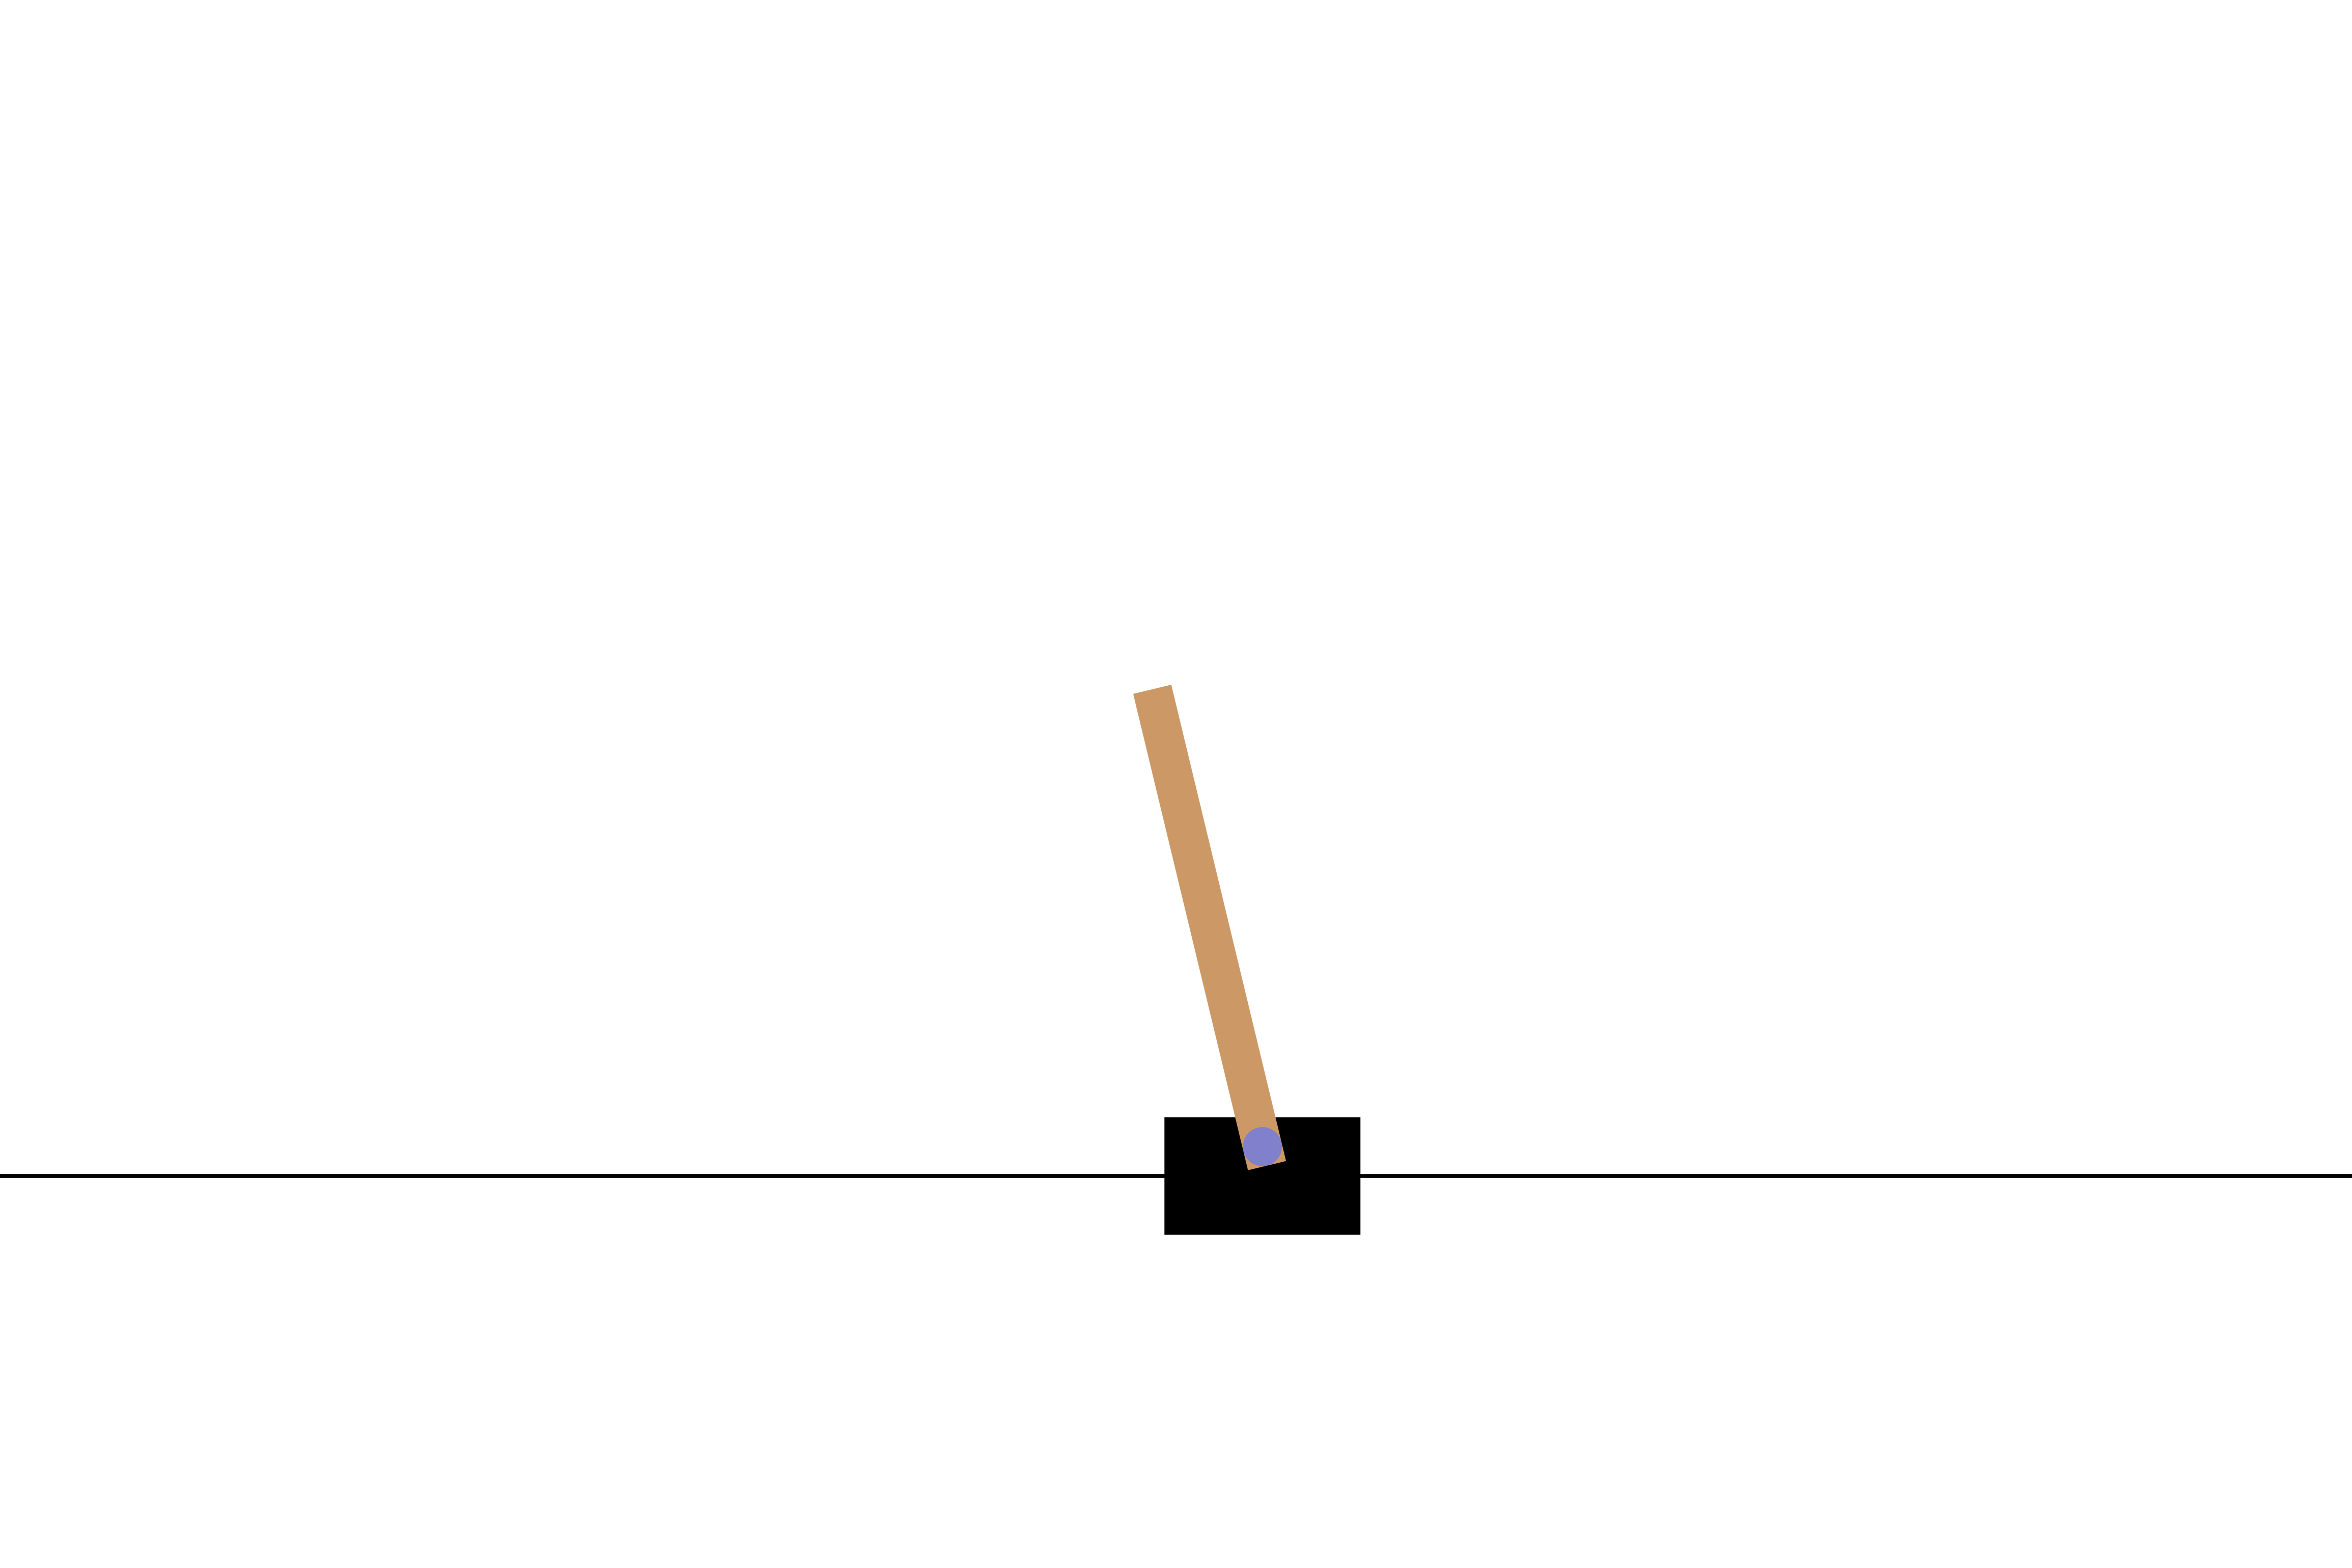
\includegraphics[width=0.75\textwidth]{cartpole.png}
    }
    \caption[
        The cart-pole environment in OpenAI Gym.
    ]{
        The cart-pole environment in OpenAI Gym.
        An agent must move the cart to the right or the left to combat gravity and keep the pole upright.
        If the pole falls over or the cart moves too far from the centre, the game is over.
        The goal is to last as long as possible.
    }
    \label{fig:cartpole}
\end{figure}

\subsection{Learning Markov decision processes}
One key concept in MDPs is the notion of value functions.
A value function is a function that estimates the expected cumulative reward from a given state or state-action pair, under a given policy.
Specifically, the state-value function $V^{\pi}(s)$ estimates the expected cumulative reward from state $s$, under policy $\pi$.
It is given by
\begin{equation}
    V^{\pi}(s) = \mathbb{E}_\pi \left[ G_t | S_t = s \right],
\end{equation}
where the expectation is taken over the distribution of future rewards and states, given that the agent is in state $s$ at time $t$.

Alternatively, one may consider a state-action value function $Q^{\pi}(s, a)$, which estimates the expected cumulative reward from state $s$, given that the agent takes action $a$, under policy $\pi$ for future steps.
It can be expressed as
\begin{equation}
    Q^{\pi}(s, a) = \mathbb{E}_\pi \left[ G_t | S_t = s, A_t = a \right].
\end{equation}

Naturally, it is desirable to maximise either, leading to the Bellman equations, from which the optimal policies can be derived.
This is alas rarely possible exactly; even if the mechanics of the game is known exactly a prior (like in card games or chess), the state spaces will generally be too large to be able to compute the value functions exactly.
Instead, one must resort to approximate methods, such as dynamic programming, Monte Carlo tree-search, and temporal difference learning.

There are three main categories of reinforcement learning algorithms:
\begin{description}
    \item[Value-based algorithms]
        The state-value function or the action-value function is learnt and then used to determine the optimal policy.
        Value-based algorithms can be very effective in problems with large state spaces, as they inherently extract the most important features of the state.
        This also makes them good at generalising to unseen states without requiring too many samples, and they can benefit from data obtained earlier in the training process with an old policy.
        They can nonetheless be sensitive to the choice of hyperparameters and may struggle with problems with continuous action spaces.


    \item[Policy-based algorithms]
        A policy, either a deterministic or stochastic mapping from states to actions, that maximises the expected cumulative reward, is learnt directly.
        This is done by defining some parametric policy $\pi_\theta(a | s)$, where $\theta$ is a vector of parameters, and then optimising the parameters $\theta$ given the data collected from the agent's interactions with the environment thus far.
        Policy-based algorithms are well suited for problems with continuous action spaces, as their parametric mappings will naturally produce continuous actions.
        Their inherent stochasticity also makes them well suited for exploration, as they will naturally explore different actions, also making them more robust to noise and environmental randomness.
        They can easily converge to local minima, which may be good enough in some cases, but also make it hard to train them as well as is desired.

    \item[Model-based algorithms]
        These algorithms learn a model of the environment, including the transition probabilities and rewards, and then use this model to plan and optimise the agent's behaviour.
        Model-based algorithms can be very effective in problems where the environment is predictable, and the agent can simulate different action sequences to find the optimal policy.
        However, these algorithms can be computationally expensive and may require a large amount of data to learn an accurate model.

\end{description}

It is primarily the model-free, latter two methods (or combinations thereof) that have seen the most success in recent years, and these which will be discussed further in \cref{sec:rl_algs}.
But also model-based algorithms have seen some commendable results recently, for example, playing \textit{Minecraft}~\autocite{minecraft} and being able to find diamonds~\autocite{hafner2023}.


\subsection{Difficulties}
\label{sec:difficulties}
The exploration-exploitation dilemma as discussed in \cref{chap:bandits} is also central to reinforcement learning.
To learn an optimal policy, an agent needs to explore the environment to discover new and potentially rewarding actions, while at the same time exploiting the actions that are already known to be rewarding.
Balancing exploration and exploitation is a difficult problem, and many RL algorithms use heuristic exploration strategies or rely on random noise to encourage exploration.

Another challenge in RL is the problem of credit assignment.
The credit assignment problem refers to the difficulty of assigning credit to the actions that lead to a particular reward.
In some cases, the reward may be delayed, making it difficult to determine which actions led to the reward.
This problem is especially pronounced in environments with long time horizons, where the actions taken early in the episode may have a significant impact on the final reward.

Designing appropriate rewards is a critical component of reinforcement learning, as they guide the agent's behaviour towards achieving the desired outcome.
However, poorly designed rewards can lead to slow or intractable learning, as the agent may not receive sufficient feedback on its actions to adjust its policy.
A classic example thereof is pausing the game in \textit{Tetris} as not to lose the game~\autocite{murphy2013}.

Specialised rewards that provide more detailed feedback and guidance can improve learning, but they also make it harder to generalise to new situations.
For instance, the Atari game \textit{Montezuma's Revenge}~\autocite{montezuma} is nigh impossible to solve with off-the-shelf methods and without specialising the rewards~\autocite{salimans2018}.
While the suite of Atari games is mostly solvable with the same algorithms, the lack of immediate rewards leaves agents clueless as to how to progress.
Implementing the necessary guidance can not only be demanding, but it also loses the general applicability that is so central to RL.

RL is fundamentally more challenging than supervised learning because it requires an agent to explore and interact with its environment to learn from experience, as opposed to having access to labelled data.
Randomly discovering an optimal strategy can be highly unlikely, especially in high-dimensional state and action spaces, making it necessary to develop specialised algorithms~\autocite{sutton2018}.
While humans can employ prior knowledge, such as that keys will open doors, reinforcement learning agents typically have to learn this by chance.
In a testing video game, the removal of non-essential visual elements, altering the orientation and employing unconventional control schemes had minimal impact on RL algorithms, whereas it caused a drastic shift for humans, going from completing the game much faster than the RL algorithms to being unable to complete the game whatsoever~\autocite{dubey2018}.
It can be computationally expensive and require significant amounts of data to learn an optimal policy, which is why the idea of algorithms competing against themselves has been so central in achieving super-human performance in board and video games~\autocite{silver2016}.
All this leads to the necessity of deep learning in reinforcement learning.
Before those methods can be explained, the general concept of deep learning needs to be discussed, namely the artificial neural network.